\documentclass{article}
\usepackage{graphicx}
\graphicspath{{res/}}
\usepackage{subcaption}

\title{ Latex Figures}
\date{2020/11/09}
\author{Steven Huang}

\begin{document}
\pagenumbering{gobble}
\maketitle
\newpage
\pagenumbering{arabic}

\section{figure1}
Hello World!
\section{figure2}
\begin{figure}[h!]
  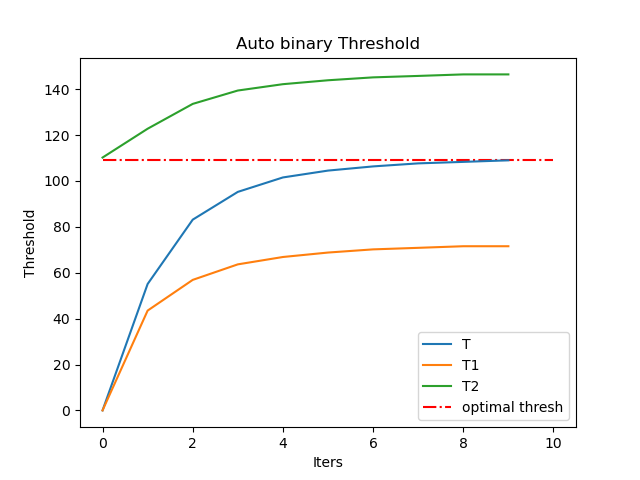
\includegraphics[width=\linewidth]{autoThres.png}
  \caption{Auto binary threshold method.}
  \label{fig:bin1}
\end{figure}

\begin{figure}[h!]
  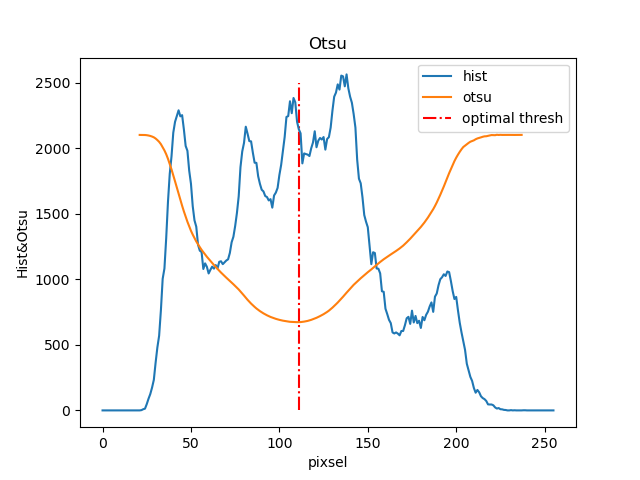
\includegraphics[width=\linewidth]{otsu.png}
  \caption{Otsu threshold method.}
  \label{fig:Otsu1}
\end{figure}

Figure \ref{fig:bin1} shows a boat. 
Figure \ref{fig:Otsu1} shows the otsu method.

\section{sub-figure1}
Here will show tow images next to each other.

\begin{figure}[h!]
  \centering
  \begin{subfigure}[b]{0.45\linewidth}
    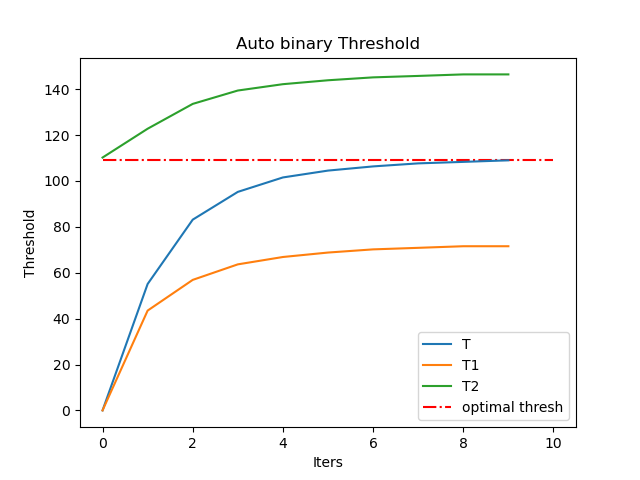
\includegraphics[width=\linewidth]{autoThres.png}
    \caption{Auto threshold.}
  \end{subfigure}
  \begin{subfigure}[b]{0.45\linewidth}
    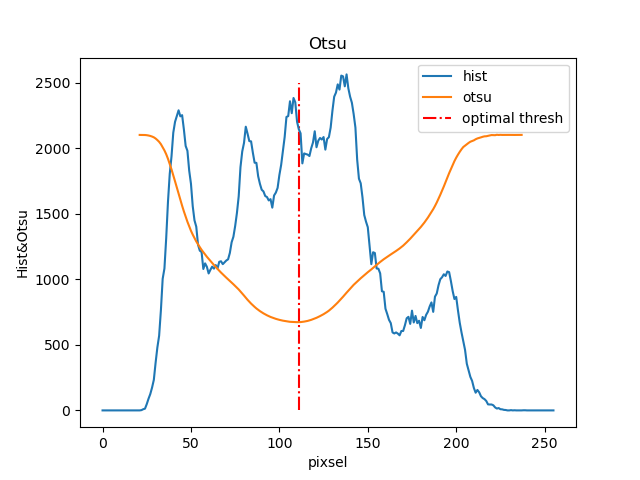
\includegraphics[width=\linewidth]{otsu.png}
    \caption{Otsu method.}
  \end{subfigure}
  \caption{The method for image binary segmentation.}
  \label{fig:imageSeg}
\end{figure}

\section{sub-figure2}
More conloex align figures.
\begin{figure}[h!]
  \centering
  \begin{subfigure}[b]{0.4\linewidth}
    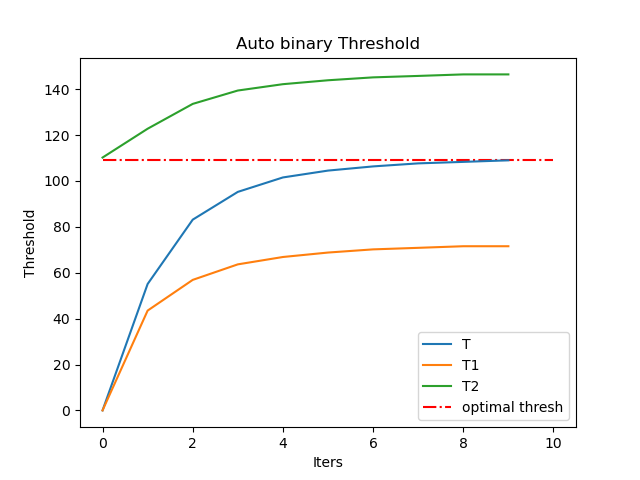
\includegraphics[width=\linewidth]{autoThres.png}
     \caption{Coffee.}
  \end{subfigure}
  \begin{subfigure}[b]{0.4\linewidth}
    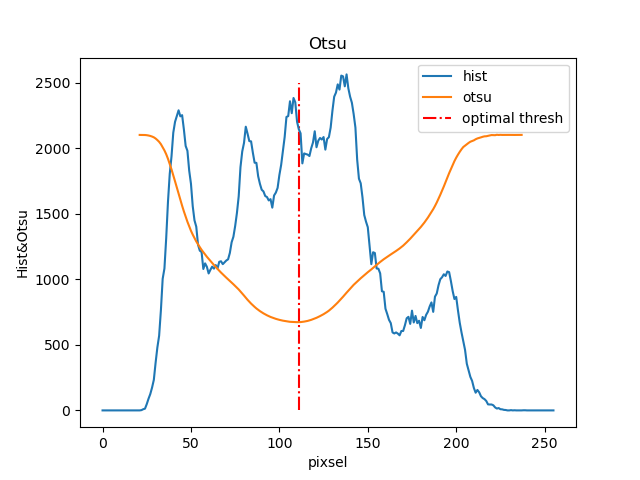
\includegraphics[width=\linewidth]{otsu.png}
    \caption{More coffee.}
  \end{subfigure}
  \begin{subfigure}[b]{0.4\linewidth}
    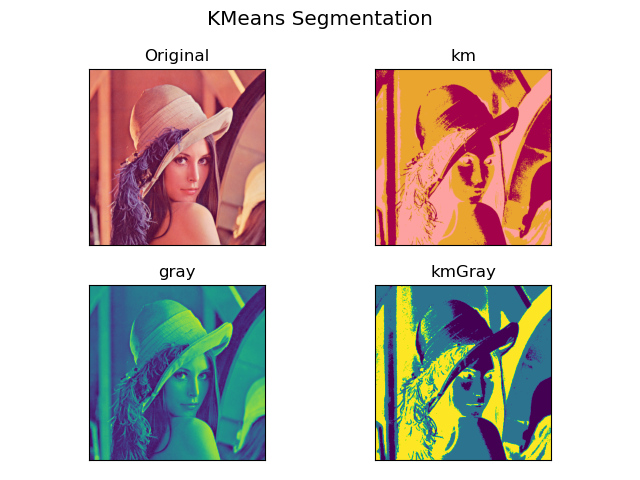
\includegraphics[width=\linewidth]{kMeans.png}
    \caption{Too much coffee.}
  \end{subfigure}
  \begin{subfigure}[b]{0.4\linewidth}
    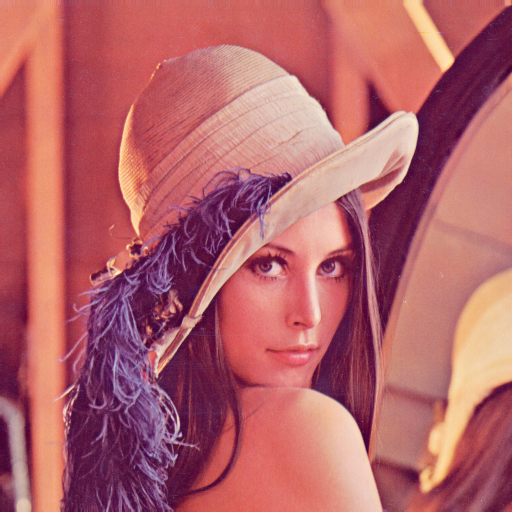
\includegraphics[width=\linewidth]{Lenna.png}
    \caption{Too much coffee.}
  \end{subfigure}
  \caption{The same cup of coffee. Multiple times.}
  \label{fig:coffee3}
\end{figure}

\end{document}